\begin{savequote}[75mm]
You are like my father in some ways.\\
WHAT RESEMBLANCE DO YOU SEE\\
You are not very aggressive but I think you don't want me to notice that.\\
WHAT MAKES YOU THINK I AM NOT VERY AGGRESSIVE
\qauthor{A conversation with ELIZA (from \citet{weizenbaum1966eliza})}
\end{savequote}
\chapter{Question Generation and Answering}

\section{Introduction}

In this chapter, I describe how the Luna Rating System fits within the broader context of existing AI research. LRS invites direct applications of two subfields of Natural Language Processing: Question Generation (QG) and Question Answering (Q\&A). QG considers the automatic generation of questions, typically derived from natural language or structured input. The Interview Phase of the Luna Game, in which players must compose original questions and reason about expected answers, is a straightforward application of QG. Q\&A is the complementary study of answering natural language questions automatically. The Response Phase, which requires each player to answer the questions of the other player, similarly corresponds to Q\&A. (The Guess Phase does not have an obvious corollary problem in existing research, but its structure suggests an intriguing new problem, which I characterize in Chapter $5$.) The large bodies of work on QG and Q\&A can be directly incorporated into LRS. Here I offer a brief review of both problems and discuss their applicability to LRS. 

\section{Question Generation}

\subsection{Problem Scope}

Question Generation, as the name suggests, is the study of automatically generating linguistically valid questions. In practice, a collection of natural language samples is provided as input, and questions pertaining to that text are produced as output \citep{rus2011question, heilman2011automatic}. These text samples may be relatively short, like a single sentence \citep{ali2010automatic, rus2011question}, or longer, like a paragraph \citep{mannem2010question} or a full natural language corpus \citep{heilman2011automatic}. They may be factual, like the encyclopedia examples, or fictional, like a short story derived from a simulated world \citep{weston2015towards}. This variety has resulted in a field that is fairly fragmented, despite attempts to cement the problem's scope \citep{piwek2008generating}. As it stands, the one commonality among all work on QG is the ambition to automatically generate an abundance of human-like questions. 
 
\subsection{Research Motivation}

Research in QG is often motivated by the prospect of automated intelligent educational tools \citep{graesser2005scaffolding, heilman2011automatic}. A system capable of generating a set of reasonable questions from an academic text would be invaluable for learning and assessment, especially in the era of MOOCs and other online educational resources. Heilman's work, which I describe in more detail below, is primarily motivated by this educational potential \citep{heilman2011automatic}. In the specific context of English language learning, \citet{kunichika2004automated} create an interactive system that generates questions from a novice textbook and then adaptively presents a series of questions to students based on their previous responses. \citet{xu2009automatic} provide a similar game-based system for learning Mandarin. Other motivations for QG include assisting human questioning, participating in general dialogue \citep{walker2001spot}, and providing synthetic datasets for the related task of Q\&A \citep{1603.06807}. \citet{piwek2008generating} make a broad case for QG as a task of interest for AI and Computational Linguistics, advocating an ``open-minded approach... [towards] a new and hopefully soon burgeoning area of research."

\subsection{Shared Task}

In $2010$, the Question Generation Shared Task and Evaluation Challenge (QGSTEC) was announced, leading to a modest uptick of interest on the problem \citep{rus2011question}. QGSTEC includes two tasks: QG from sentences, and QG from paragraphs. In both cases, the questions generated by contestants are evaluated by human judges on the basis of relevance, question type, correctness, ambiguity, and variety. The centralized challenge succeeded in soliciting five entrants \citep{ali2010automatic,pal2010qgstec,yao2010question, vargaha, mannem2010question}. Beyond 2010, the impact of QGSTEC has been minimal, likely due in part to the limitations of human-dependent evaluation. To my knowledge, no other shared tasks have been proposed to take its place. Subsequent new methods for QG are instead benchmarked by direct comparison with reimplemented old methods on new datasets \citep{1603.06807}.

\subsection{Existing Methods}

If surface-level questions suffice, and questions need not be diverse in style, there are several simple QG options available. One coarse approach is the Cloze procedure, in which words from the input text are randomly replaced with blanks for the responder to complete \citep{taylor1953cloze}. For example, the input text ``George Washington was born in Virginia'' might generate the question ``George Washington was born in $\rule{2cm}{0.05mm}$''. The next level of sophistication involves applying templates to text in search of specific syntax patterns, and then applying one of several predefined transformations accordingly. For example, the previous input text might be matched and transformed to the question ``Where was George Washington born?'' or ``Who was born in Virginia?'' \citep{gates2008automatically, kunichika2004automated, heilman2011automatic}. A variant of this template-based strategy is employed by ELIZA, the therapist-like chatterbot developed in $1966$ by Weizenbaum \citep{weizenbaum1966eliza}. Template-based methods may also be used to generate multiple choice questions \citep{mitkov2006computer}. Work by \citet{ali2010automatic} relies on sentence classification and syntax parsing before applying transformations to generate questions.  \citet{wang2007automatic} use a similar transformation-based procedure in the domain of medical texts. While template methods produce syntactically correct questions that are more appropriate for applications like dialogue, it is not necessarily the case that they produce deeper semantics than the simpler Cloze procedure.

More sophisticated methods for QG utilize machine learning techniques. One way to convert QG into an instance of a known machine learning problem is by \textit{overgenerating transformations and ranking} \citep{heilman2010extracting, heilman2010good, heilman2011automatic, mannem2010question}. This two-step process begins with a template-based question generation method, which is applied liberally to create a surplus of syntactically valid questions. Next, a learned ranking function sorts the questions in order of semantic goodness. The top ranked questions are returned as the final output. This paradigm is an attractive approach to QG, since it separates the task of generating all syntactically possible questions from the task of selecting semantically valid and useful questions. In Heilman's work, the overgeneration step is accomplished through syntax pattern matching and manually encoded transformation rule applications. Ranking is then performed using a variety natural language features. The ranking step is shown to double the acceptability of generated questions, as defined by human judges \citep{heilman2011automatic}. 

A potential breakthrough in QG was announced extremely recently by \citet{1603.06807}. Taking inspiration from the encoder-decoder paradigm in Deep Learning for machine translation \citep{cho2014learning}, this work uses Recurrent Neural Networks to generate questions word-by-word based on input facts from the Freebase knowledge base \citep{bollacker2008freebase}. The 30 million factoid questions generated outperform template-based methods on all metrics, and are reportedly ``indistinguishable'' from human questions from the perspective of human judges. This work is notable not only for the records it breaks, but also for the senior author on the paper, Yoshua Bengio, who is one of the pioneers of Deep Learning. If the Deep Learning research community follows his lead on the problem, QG is likely to soon enjoy a wave of renewed research interest.

\subsection{Evaluation Metrics}

All previous work on QG is reliant to certain extents on manual human input for evaluation \citep{rus2011question, heilman2011automatic, 1603.06807}. Human judges are typically asked to indicate whether or not the generated questions are syntactically and semantically sensible \citep{rus2011question}. The quality of questions is not usually evaluated beyond this binary validation. Indeed, finer grained evaluation would likely be vulnerable to subjective variation among judges. With judgments acquired, research has varied on the exact metric reported. For example,  \citet{ali2010automatic} seek to maximize the total number of valid questions generated, while \citet{heilman2011automatic} aims to maximize the \textit{fraction} of valid questions over the entire generated set. The recent work by \citet{1603.06807} reports both the total and fraction of valid questions according to human evaluators. However, the authors also propose several methods for automatic human-independent evaluation based on metrics used in machine translation and sentence similarity.  It remains to be seen whether these metrics will be accepted and adopted in future work. Up until this point, the challenge of defining a metric that is both semantically meaningful and efficiently evaluated has arguably been the greatest obstacle for QG research.

\subsection{Luna and Question Generation}

Any of the described QG methods could easily be used to generate questions for the Interview Phase of a Luna Game. In fact, questions could be directly selected from the publicly available outputs of these methods (e.g. the 30 million questions generated by \citet{1603.06807}). However, for the purpose of playing the Luna Game, not all questions are generated equal. Factoid questions, for example, are unlikely to yield informative responses from human opponents, since external resources may be referenced in the course of a game. Questions generated from fictional text may be more revealing, though the fictional text itself would need to be provided as part of the question. Of course, a player who is interested solely in the response component of the Luna Game may only care about question selection insofar as it disguises the player's identity from repeat opponents. In this case, any of the QG methods will likely serve the player's purpose.

The relationship between QG and LRS is also promising in the other direction: LRS could prove beneficial to QG researchers who wish to assess their methods. As discussed above, progress on QG has been significantly hindered by the lack of quantitative metrics for question quality. Smarts Ratings and Luna Game guesses could be seen as signals of question quality; questions that tend to lead to guesses close to actual Smarts Ratings are informative.  This notion of question informativeness is important, especially in the context of automatic intelligent tutoring, and otherwise difficult to quantify. Moreover, the questions that are naturally produced by human players in LRS could chart the course for future work in QG, which ultimately aims to automatically generate human-like questions.

\section{Question Answering}

\subsection{Problem Scope}

Q\&A is defined as the general problem of automatically responding to any question posed in natural language \citep{andrenucci2005automated, hirschman2001natural}. The breadth of the problem can be a blessing and a curse. Such a broad definition effectively encompasses all of AI; it is argued that the problem can only be solved by a machine with true general AI \citep{yampolskiy2013turing}. This completeness is what makes Q\&A an appropriate centerpiece in a test for AI. At the same time, the tremendous scope of the problem can be a barrier to progress. The lack of common structure among possible questions gives researchers little to exploit. Moreover, the task of assessing a candidate solution to Q\&A presents several challenges and ambiguities. How should test questions be selected from the extraordinarily large number of possible question topics and forms? How should answers be assessed, especially in the case that a question may be subjective, or have several equally valid answers? These difficult questions have discouraged research on the general Q\&A problem in favor of more narrow tasks.

In pursuit of tractability, researchers have explored a variety of restrictions on Q\&A. These restrictions may apply to question content, question format, or answer format. Question content may be limited by focusing on a fixed source of information that assumedly contains all answers. The size and structure of this source can greatly influence the difficulty of the task. In one extreme, the source might be all of Wikipedia in natural language form, with no further direction nor additional parsing provided. An easier source would be a structured knowledge base like Freebase, which organizes relational information in a very precise and predictable way \citep{bollacker2008freebase}. The source may also be small and question-specific, e.g. a reading comprehension task that supplies text samples and asks the reader to infer answers based only on the samples \citep{richardson2013mctest}. With a source established, question formats are often limited so that there is a clear single correct answer. For example, the questions may be true or false, multiple choice, or single word answers. The answers themselves may be further limited to natural language fragments, or even single words, that are lifted directly from the provided text. Each of these potential restrictions on Q\&A represents a tradeoff between tractability and generalizability. As the field progresses, the range of what is tractable has expanded, allowing for commensurate improvements on more general problems.

\subsection{Research Motivation}

The motivation for Question Answering is abundant and self-evident. Every problem in AI --- in all fields, in fact --- can be phrased as a question. Imagine a machine that could answer every possible question. It could be asked, for example, ``What are the answers to all possible questions, ordered by importance to humanity?'' Of course, practical research on Q\&A is driven by much more immediate ambitions. Q\&A is often presented within the context of the World Wide Web and restricted to factual questions \citep{cucerzan2005factoid, ravichandran2002learning, kwok2001scaling}. A web-based system capable of directly answering user queries would be the prize possession of a search engine company. Indeed, with the introduction of Knowledge Panels with search responses that are derived from the Knowledge Graph, Google is increasingly blurring the lines between Information Retrieval and Q\&A \citep{singhal2012introducing}. Another extrinsic, if toy motivation for Q\&A is the television trivia game Jeopardy!, which inspired IBM's DeepQ\&A team to develop IBM Watson, perhaps the most famous Q\&A system to date \citep{ferrucci2012introduction}. Additionally, personal assistant technologies, like the DARPA PAL project (which later became Apple's Siri) and the Amazon Echo, all rely on Q\&A for their core functionality \citep{aron2011innovative, tsiao2007natural}. The corporate origin of each of these examples is representative; there is enormous product-driven demand for progress on Q\&A.

\subsection{Shared Tasks}

In $1999$, a Q\&A task was added to the Text Retrieval Conference (TREC), an ongoing series of workshops in information retrieval that provides centralized benchmarks for many similar problems \citep{voorhees1999trec}. The dataset used for the task consists of $200$ factoid short-answer questions, such as ``How many calories are there in a Big Mac?'', and provides a natural language corpus of newspaper articles and similar archives that somewhere contain the answers. The answers provided by the algorithms are assessed by human judges for validity, representing the same bottleneck of the Question Generation task discussed above. Nonetheless, the Q\&A TREC task, which was repeated every year from $1999$ to $2007$, consistently enjoyed far more attention than the analogous QG task \citep{dang2007overview}. Indeed, the concentration of $21$st century Q\&A research around the factoid free text subproblem is likely due in part to the prominence of the TREC task \citep{hirschman2001natural}.

Recent work by Facebook AI could potentially serve as an epicenter for research on the non-factoid subproblem. In a paper titled \textit{Towards AI-Complete Question Answering: A Set of Prerequisite Toy Tasks}, \citet{weston2015towards} define $20$ simplified non-factoid question answering subtasks, forming the bAbI task. The subtasks are designed to strip away many of the superfluous complexities of naturally occurring text, instead focusing on core concepts one-by-one. Questions are presented with a collection of statements containing the desired answer. For example, the simplest type of question is the Single Supporting Fact, in which the answer may be derived directly from a single provided statement. All questions in bAbI are based on a simulated world involving several agents and objects with various possible actions. In relying on a simple simulation, as did Winograd in earlier work \citep{winograd1971procedures}, bAbI is able to provide an ideal amount of unpredictability while still keeping the task focused on specific types of questions. The bAbI task has already inspired advances in Deep Learning approaches to Q\&A, including the notable introduction of Memory Networks \citep{sukhbaatar2015weakly}.

\subsection{Existing Methods}

Q\&A has been studied consistently for over half a century. The majority of work on the subject falls into one of three categories: factoid Q\&A from structured knowledge bases, factoid Q\&A from free text, and non-factoid Q\&A. Given a structured knowledge base, i.e. a list of logical predicates, Q\&A essentially reduces to the subproblem of mapping natural language to queries, either explicitly or with the addition of a latent term \citep{yao2014information, zelle1996learning}. With multiple possible answers, an additional selection step is required, which usually involves a ranking function similar to those used for Question Generation. Factoid Q\&A from free text cannot take advantage of structured relations, and thus has the additional burden of parsing text from a natural language corpus in search of relevant information \citep{ravichandran2002learning}. While this added challenge is considerable, these algorithms typically also have access to significantly more data than their knowledge base oriented counterparts \citep{brill2001data, hermann2015teaching}. This setup makes the factoid Q\&A from free text especially appropriate for Deep Learning techniques. Both types of factoid Q\&A leave open the possibility of training an algorithm on an external dataset of facts before the questions are asked. In contrast, non-factoid Q\&A forces an algorithm to discover answers to questions on an ad-hoc basis \citep{soricut2004automatic}. Non-factoid Q\&A typically includes a fictional story as part of the prompt, and then ask a question which has an answer that can only be inferred from the story. While the information retrieval portion of the task is somewhat simplified, the challenges of automatic reasoning and inference are brought to the fore.

Another distinguishing feature among approaches to Q\&A is the extent to which questions and answers are parsed into intermediate representations. Recent efforts have attempted to learn mappings directly from questions to answers without forming any representations in between. Before the rise of Deep Learning, such efforts would have been unthinkable due to the incredibly large space of possible questions and answers in any practical domain \citep{hirschman2001natural}. For example, Figure \ref{fig:NLPQA}, reproduced from \citep{androutsopoulos1995natural}, provides an example of how an end-to-end system for Q\&A was divided into modules in $1995$. The system includes modules for syntax parsing, semantic rule application, database querying, and output generation, each which must be separately addressed. A $2001$ review by Burger et al. divides Q\&A even further into $12$ subproblems, including Question Classes, Question Processing, Context, Data Sources, Answer Extraction, and Answer Formulation among others \citep{burger2001issues}. The current state of the art suggests that this level of granularity does not necessarily lead to better performance.  

\begin{figure}[h]
\centerline{%
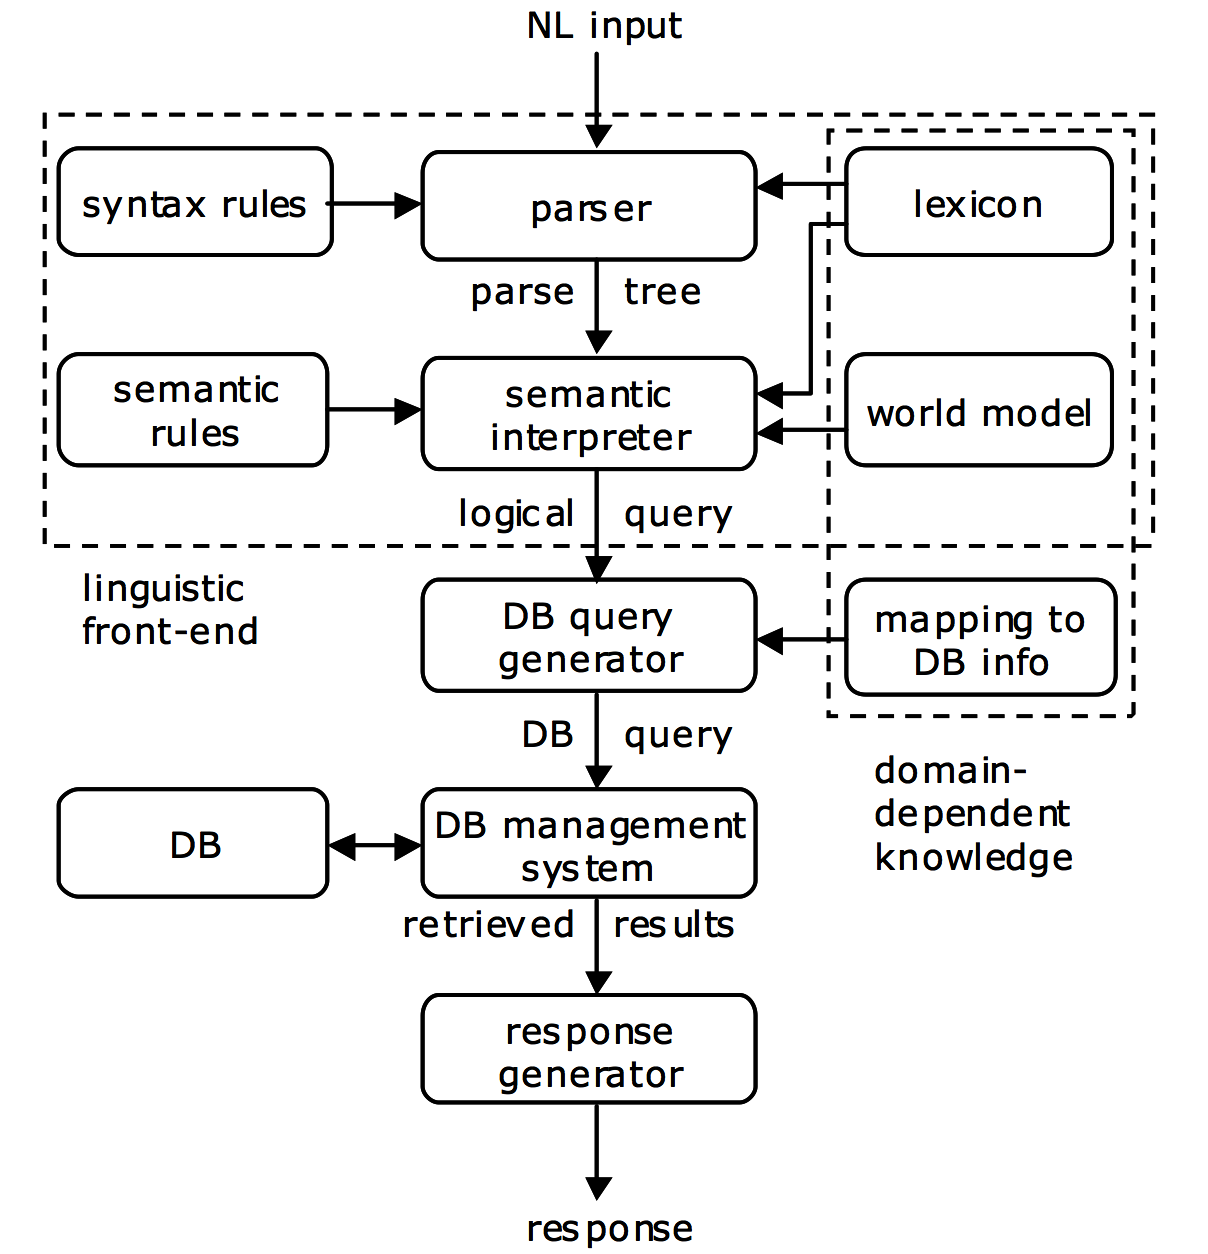
\includegraphics[width=0.5\textwidth]{figures/NLPQA.png}}%
\caption{Architecture of a typical Natural Language system for Question Answering in $1995$, from \citep{androutsopoulos1995natural}. Some modern approaches eschew intermediate representations and attempt to produce answers directly from inputs.}
\label{fig:NLPQA}
\end{figure}


\subsection{Luna and Question Answering}

Q\&A is the research problem that is most intimately related to LRS. At its core, LRS is a benchmark for Q\&A. Performance in the Interview and Guess Phases of the Luna Game does not affect the Smarts Rating of the player; only the Response Phase determines the rating. Thus only the Response Phase, and the Q\&A problem it represents, matter for the purpose of judging AI with LRS. The Q\&A methods reviewed in this chapter may be used directly during the Response Phase. Of course, a Q\&A method for factoid questions will not fare well on non-factoid questions, nor vice versa. By design, LRS favors methods that are comprehensive and generalized. Nonetheless, the performance of a narrowly scoped method in LRS will be revealing of that method's significance beyond its scope. The maximum performance of a Q\&A method in LRS will illuminate the distance between current AI research and its ultimate target.



\section{Conclusion}

This review of Question Generation and Question Answering demonstrates that the Luna Rating System does not exist in isolation from existing AI research. Rather, LRS can be seamlessly integrated into ongoing research on both of these problems, Q\&A in particular. The recent work presented here indicates research interest not only in Q\&A, but also in methods to steer research on the problem towards generality. The fact that a mainstream publication includes ``Towards AI-Complete Question Answering'' in its title is evidence of this trend. The Luna Rating System offers another path towards AI-Complete Question Answering --- a path that complements bAbI and requires no deviation from the current trajectory of the research community.

%\section{Response Phase: an Application of Question Answering}
%
%\subsection{Scope of Question Answering}
%
%The Response Phase of the Luna Game bears immediate resemblance to a subfield of Natural Language Processing known as Question Answering (Q\&A). Q\&A is defined as the general problem of automatically responding to any question posed in natural language \citep{andrenucci2005automated, hirschman2001natural}. The breadth of the problem can be a blessing and a curse. Such a broad definition effectively encompasses all of artificial intelligence; it is argued that the problem can only be solved by a machine with true general AI \citep{yampolskiy2013turing}. This completeness is what makes Q\&A an appropriate centerpiece in a test for AI. At the same time, the tremendous scope of the problem can be a barrier to progress. The lack of common structure between possible questions gives researchers little to exploit. Moreover, the task of assessing a candidate solution to Q\&A presents several challenges and ambiguities. How should test questions be selected from the extraordinarily large number of possible question topics and forms? How should answers be assessed, especially in the case that a question may be subjective, or have several equally valid answers? These difficult questions have discouraged research on the general Q\&A problem in favor of more narrow tasks.
%
%In pursuit of tractability, researchers have explored a variety of restrictions on Q\&A. These restrictions may apply to question content, question format, or answer format. Question content may be limited by focusing on a fixed source of information that assumedly contains all answers. The size and structure of this source can greatly influence the difficulty of the task. In one extreme, the source might be all of Wikipedia in natural language form, with no further direction nor additional parsing provided. An easier source would be a structured knowledge base like Freebase, which organizes relational information in a very precise and predictable way \citep{bollacker2008freebase}. The source may also be small and question-specific, e.g. a reading comprehension task that supplies text samples and asks the reader to infer answers based only on the samples \citep{richardson2013mctest}. With a source established, question formats are often limited so that there is a clear single correct answer. For example, the questions may be true or false, multiple choice, or single word answers. The answers themselves may be further limited to natural language fragments, or even single words, that are lifted directly from the provided text. Each of these potential restrictions on Q\&A represents a tradeoff between tractability and generalizability. As the field progresses, the range of what is tractable has expanded, allowing for commensurate improvements on more general problems.
%
%\subsection{Previous Work on Question Answering}
%
%The motivation for Question Answering is abundant and self-evident. Every problem in AI --- in all fields, in fact --- can be phrased as a question. Imagine a machine that could answer every possible question. It could be asked, for example, ``What are the answers to all possible questions, ordered by importance to humanity?'' Of course, practical research on Q\&A is driven by much more immediate ambitions. Q\&A is often presented within the context of the World Wide Web and restricted to factual questions \citep{cucerzan2005factoid, ravichandran2002learning, kwok2001scaling}. A web-based system capable of directly answering user queries would be the prize possession of a search engine company. Indeed, with the introduction of Knowledge Panels with search responses that are derived from the Knowledge Graph, Google is increasingly blurring the lines between Information Retrieval and Q\&A \citep{singhal2012introducing}. Another extrinsic, if toy motivation for Q\&A is the television trivia game Jeopardy!, which inspired IBM's DeepQ\&A team to develop Watson, perhaps the most famous Q\&A system to date \citep{ferrucci2012introduction}. Additionally, personal assistant technologies, like the DARPA PAL project (which later became Apple's Siri) and the Amazon Echo, all rely on Q\&A for their core functionality \citep{aron2011innovative, tsiao2007natural}. The corporate origin of each of these examples is representative; there is enormous product-driven demand for progress on Q\&A.
%
%Q\&A has been studied consistently for over half a century. The majority of work on the subject falls into one of three categories: factoid Q\&A from structured knowledge bases, factoid Q\&A from free text, and non-factoid Q\&A. Given a structured knowledge base, i.e. a list of logical predicates, Q\&A essentially reduces to the subproblem of mapping natural language to queries, either explicitly or with the addition of a latent term \citep{yao2014information, zelle1996learning}. With multiple possible answers, an additional selection step is required, which usually involves a ranking function similar to those used for Question Generation. Factoid Q\&A from free text cannot take advantage of structured relations, and thus has the additional burden of parsing text from a natural language corpus in search of relevant information \citep{ravichandran2002learning}. While this added challenge is considerable, these algorithms typically also have access to significantly more data than their knowledge base oriented counterparts \citep{brill2001data, hermann2015teaching}. This setup makes the factoid Q\&A from free text especially appropriate for Deep Learning techniques. Both types of factoid Q\&A leave open the possibility of training an algorithm on an external dataset of facts before the questions are asked. In contrast, non-factoid Q\&A forces an algorithm to discover answers to questions on an ad-hoc basis \citep{soricut2004automatic}. Non-factoid Q\&A typically includes a fictional story as part of the prompt, and then ask a question which has an answer that can only be inferred from the story. While the information retrieval portion of the task is somewhat simplified, the challenges of automatic reasoning and inference are brought to the fore.
%
%Another distinguishing feature among approaches to Q\&A is the extent to which questions and answers are parsed into intermediate representations. Recent efforts have attempted to learn mappings directly from questions to answers without forming any representations in between. Before the rise of Deep Learning, such efforts would have been unthinkable due to the incredibly large space of possible questions and answers in any practical domain \citep{hirschman2001natural}. For example, Figure \ref{fig:NLPQA}, reproduced from \citep{androutsopoulos1995natural}, provides an example of how an end-to-end system for Q\&A was divided into modules in $1995$. The system includes modules for syntax parsing, semantic rule application, database querying, and output generation, each which must be separately addressed. A $2001$ review by Burger et al. divides Q\&A even further into $12$ subproblems, including Question Classes, Question Processing, Context, Data Sources, Answer Extraction, and Answer Formulation among others \citep{burger2001issues}. The current state of the art suggests that this level of granularity does not necessarily lead to better performance.  
%
%\begin{figure}[h]
%\centerline{%
%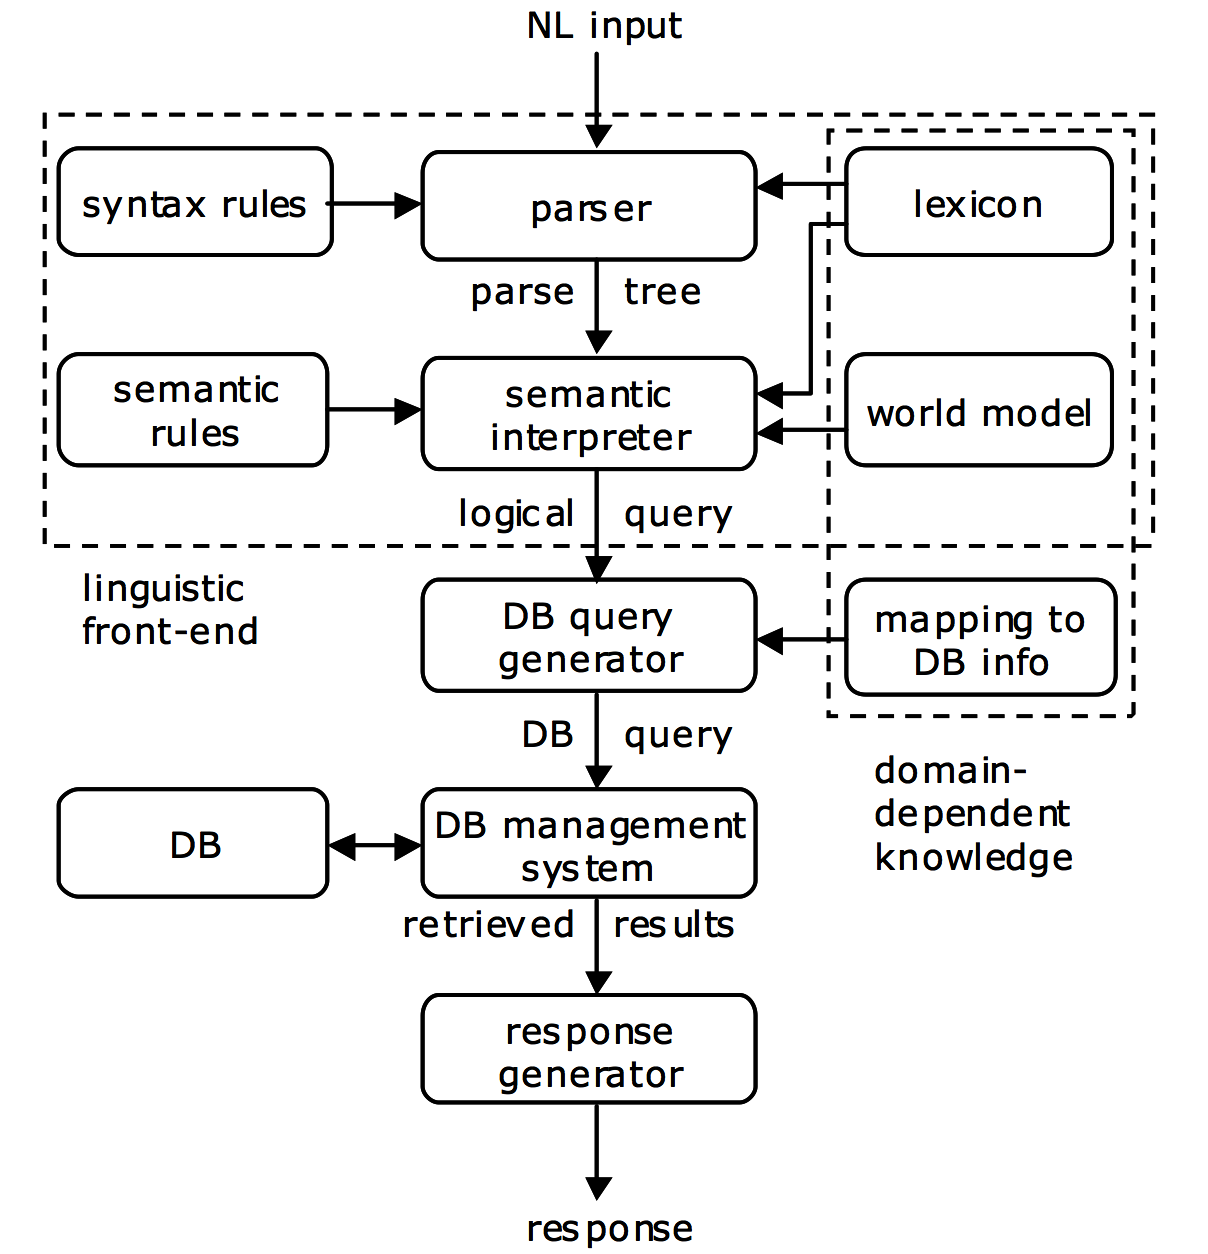
\includegraphics[width=0.5\textwidth]{figures/NLPQA.png}}%
%\caption{Architecture of a typical Natural Language system for Question Answering, from \citep{androutsopoulos1995natural}. The structure could be used in full or in part as a template for approaching the Response Problem.}
%\label{fig:NLPQA}
%\end{figure}
%
%In $1999$, a Q\&A task was added to the Text Retrieval Conference (TREC), an ongoing series of workshops in information retrieval that provides centralized benchmarks for many similar problems \citep{voorhees1999trec}. The dataset used for the task consists of $200$ factoid short-answer questions, such as ``How many calories are there in a Big Mac?'', and provides a natural language corpus of newspaper articles and similar archives that somewhere contain the answers. The answers provided by the algorithms are assessed by human judges for validity, representing the same bottleneck of the Question Generation task discussed above. Nonetheless, the Q\&A TREC task, which was repeated every year from $1999$ to $2007$, enjoyed far more attention than the analogous QG task has thus far \citep{dang2007overview}. The datasets from the task have also been utilized consistently in subsequent work and have been used as a benchmark to establish progress. Indeed, the concentration of $21$st century Q\&A research around the factoid free text subproblem is likely due in part to the prominence of the TREC task \citep{hirschman2001natural}.
%
%Recent work by Facebook AI could potentially serve as an epicenter for research on the non-factoid subproblem. In a paper titled \textit{Towards AI Complete Question Answering: A Set of Prerequisite Toy Tasks}, Weston et al. define $20$ simplified non-factoid question answering subtasks, forming the bAbI task \citep{weston2015towards}. The subtasks are designed to strip away many of the superfluous complexities of naturally occurring text, instead focusing on core concepts one-by-one. Following the non-factoid question paradigm discussed above, questions are presented with a collection of statements containing the desired answer. For example, the simplest type of question is the Single Supporting Fact, in which the answer may be derived directly from a single provided statement. All questions in bAbI are based on a simulated world involving several agents and objects with various possible actions. In relying on a simple simulation, as did Winograd in earlier work \citep{winograd1971procedures}, bAbI is able to provide an ideal amount of unpredictability while still keeping the task focused on specific types of questions. The bAbI task has already inspired advances in Deep Learning approaches to Q\&A, including the notable introduction of Memory Networks \citep{sukhbaatar2015weakly}.
%
%\subsection{Question Answering: The Way Forward}
%
%As evidenced by its inclusion in TREC, Q\&A has long been viewed as an extension of information retrieval \citep{kolomiyets2011survey}. Classical information retrieval returns a document containing relevant information in response to a query. Q\&A accepts the same type of query and returns a passage or parsed passage of relevant text from a similar source. The introduction of bAbI, with its non-factoid questions based on a simple simulated world, signifies a shift in the conception of Q\&A. Research on the problem is now reaching towards sophisticated reasoning in small worlds, as opposed to simple reasoning in large worlds. This shift is a critical step in the pursuit of AI-complete Q\&A. Simple factoid questions represent a very limited subset of the questions that a true AI will be expected to answer. As progress on the existing bAbI tasks continue, it will be expedient to gradually add more sophisticated tasks to continue to guide research.
%
%Work on bAbI has already produced algorithms that are able to handle an impressive range of question types pertaining to the small simulated world. Information retrieval efforts continue in parallel, making it possible to answer simple questions over increasingly large sets of semantics. A critical question for the future of Q\&A is how to close the gap between these two problems. One approach would be to gradually scale solutions to bAbI tasks to larger worlds. A mirrored method would be to increase the level of sophistication in the questions that information retrieval algorithms are able to answer. A third, and potentially most promising strategy, would be to explicitly bridge the divide while maintaining the distinction between the two problems. In this scenario, a machine could learn relations between a very limited number of entities, in the spirit of bAbI. It could then learn about a vast number of entities without learning new relations using traditional information retrieval. Finally, a mapping between the entities in the bAbI task and the retrieved entities could be learned, and new relations between these retrieved entities could be inferred. 

